%! Author = melek
%! Date = 9.06.2022

% Preamble
\documentclass[11pt]{article}

% Packages
\usepackage{amsmath}
\DeclareMathOperator*{\argmax}{argmax}

\usepackage{graphicx}
\usepackage{amssymb}
\usepackage{bm}

\graphicspath{ {../images/} }


% Document
\begin{document}

    \maketitle
    \setcounter{section}{11}


    \section{Exercises}

    \subsection{Question}

    Just as the return can be written recursively in terms of the first reward and itself one-step later (3.9), so can the $\lambda$-return.
    Derive the analogous recursive relationship from (12.2) and (12.1).

    \subsection*{Answer}

    \noindent Equation 12.1:

    \noindent $ G_{t_t+n} = R_{t+1} + \gamma R_{t+2}+ \gamma^2 R_{t+3} + \ldots + \gamma^{n-1} R_{t+n} + \gamma^n \hat{v}(S_{t+n}, w_{t+n-1}) $

    \noindent Equation 12.2:

    \noindent $ G_{t}^\lambda = (1-\lambda) \sum_{n=1}^{\infty} \lambda^{n-1} G_{t:t+n} $

    \hfill \break
    \noindent Let's start with expanding 12.2:

    \noindent $ G_{t}^\lambda = (1-\lambda) [ \lambda^{0} G_{t:t+1} + \lambda^{1} G_{t:t+2} + \lambda^{2} G_{t:t+3} + \ldots ] $

    \noindent $ G_{t}^\lambda = (1-\lambda) G_{t:t+1} + (1-\lambda) [ \lambda^{1} G_{t:t+2} + \lambda^{2} G_{t:t+3} + \ldots ] $

    \noindent $ G_{t}^\lambda = (1-\lambda) G_{t:t+1} +  \lambda (1-\lambda)  [ \lambda^{0} G_{t:t+2} + \lambda^{1} G_{t:t+3} + \ldots ] $

    \noindent $ G_{t}^\lambda = (1-\lambda) G_{t:t+1} +  \lambda (1-\lambda) \sum_{n=1}^{\infty} \lambda^{n-1} G_{t:t+1+n} $

    \hfill \break
    \noindent Let's not touch the left expression for now and focus on the second expression.
    We have a return of form $ G_{t:t+1+n} $ but a return of form $ G_{t+1:t+1+n} $ would be more useful.
    Let's try to express one in the form of the other.

    \noindent $ G_{t+1:t+1+n} =  R_{t+2} + \gamma R_{t+3} + \ldots + \gamma^{n-1} R_{t+1+n} + \gamma^n \hat{v}(s_{t+1+n},w_{t+n})  $ (12.1.1)

    \noindent $ G_{t:t+1+n} =  R_{t+1} + \gamma R_{t+2} + \gamma^2 R_{t+3} + \ldots + \gamma^{n} R_{t+1+n} + \gamma^{n+1} \hat{v}(s_{t+1+n},w_{t+n})  $

    \noindent $ G_{t:t+1+n} =  R_{t+1} + \gamma [R_{t+2} + \gamma R_{t+3} + \ldots + \gamma^{n-1} R_{t+1+n} + \gamma^{n} \hat{v}(s_{t+1+n},w_{t+n})]  $

    \noindent $ G_{t:t+1+n} =  R_{t+1} + \gamma G_{t+1:t+1+n}  $ (12.1.2)

    \hfill \break
    \noindent Going back and using equation (12.1.2):

    \noindent $ G_{t}^\lambda = (1-\lambda) G_{t:t+1} +  \lambda (1-\lambda) \sum_{n=1}^{\infty} \lambda^{n-1} (R_{t+1} + \gamma G_{t+1:t+1+n}) $

    \noindent $ G_{t}^\lambda = (1-\lambda) G_{t:t+1} +  \lambda (1-\lambda) \sum_{n=1}^{\infty} \lambda^{n-1} R_{t+1 }+   \lambda (1-\lambda) \sum_{n=1}^{\infty} \lambda^{n-1} \gamma G_{t+1:t+1+n} $

    \noindent $ G_{t}^\lambda = (1-\lambda) G_{t:t+1} +  \lambda (1-\lambda) \sum_{n=1}^{\infty} \lambda^{n-1} R_{t+1 }+   \gamma \lambda (1-\lambda) \sum_{n=1}^{\infty} \lambda^{n-1}  G_{t+1:t+1+n} $

    \hfill \break
    \noindent We have a geometric series of form $ ( \sum_{n=1}^{\inf} r \lambda^{n-1} = \frac{r}{1-\lambda} ) $:

    \noindent $ G_{t}^\lambda = (1-\lambda) G_{t:t+1} +  \lambda (1-\lambda)  \frac{R_{t+1}}{(1-\lambda)} +  \gamma \lambda (1-\lambda) \sum_{n=1}^{\infty} \lambda^{n-1} G_{t+1:t+1+n} $

    \noindent $ G_{t}^\lambda = (1-\lambda) G_{t:t+1} +  \lambda R_{t+1} +  \gamma \lambda (1-\lambda) \sum_{n=1}^{\infty} \lambda^{n-1} G_{t+1:t+1+n} $

    \hfill \break
    \noindent The right most expression is a lambda return:

    \noindent $ G_{t}^\lambda = (1-\lambda) G_{t:t+1} +  \lambda R_{t+1} +  \gamma \lambda G_{t+1}^\lambda $

    \hfill \break
    \noindent We can further simplify by expanding the 1-step return:

    \noindent $ G_{t}^\lambda = (1-\lambda) (R_{t+1} + \gamma G_{t+1:t+1}) +  \lambda R_{t+1} +  \gamma \lambda G_{t+1}^\lambda $

    \noindent $ G_{t}^\lambda = (1-\lambda) (R_{t+1} + \gamma \hat{v}(s_{t+1},w_{t}) ) +  \lambda R_{t+1} +  \gamma \lambda G_{t+1}^\lambda $

    \noindent $ G_{t}^\lambda = (1-\lambda) \gamma \hat{v}(s_{t+1},w_{t})  + (1-\lambda) R_{t+1} +  \lambda R_{t+1} +  \gamma \lambda G_{t+1}^\lambda $

    \noindent $ G_{t}^\lambda = (1-\lambda) \gamma \hat{v}(s_{t+1},w_{t})  + R_{t+1} +  \gamma \lambda G_{t+1}^\lambda $

    \noindent $ G_{t}^\lambda =  R_{t+1} + (1-\lambda) \gamma \hat{v}(s_{t+1},w_{t}) +  \gamma \lambda G_{t+1}^\lambda $ where $t < T-1$

    \hfill \break
    \noindent if $t \ge T-1$ then by equation 12.3:

    \noindent $ G_{t}^\lambda = G_t $



    \subsection{Question}

    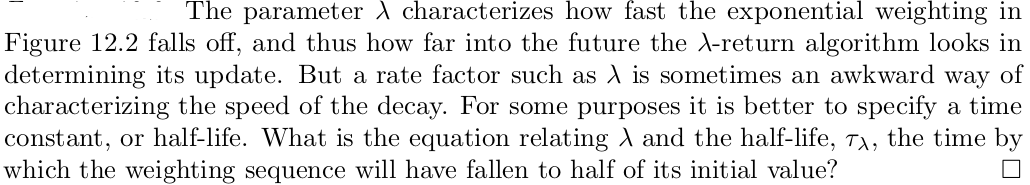
\includegraphics[scale=0.9]{exercise_12_2q}

    \subsection*{Answer}

    \noindent Half of initial weighting sequence:
    \noindent $ \frac{(1-\lambda)}{2} $

    \noindent Weighting sequence at time $t+m$:
    \noindent $ (1-\lambda) \lambda^m $

    \noindent Then by definition:
    \noindent $ (1-\lambda) \lambda^m = \frac{(1-\lambda)}{2} $

    \noindent $ \lambda^m = \frac{1}{2} $

    \noindent $ m = \log_{\lambda} \frac{1}{2} = - \log_{\lambda} 2 = \frac{\ln 2}{\ln \lambda}$

    \noindent The actual time step is:

    \noindent $ \tau_{\lambda} = t + m = t + \frac{\ln 2}{\ln \lambda} $


    \subsection{Question}

    Some insight into how $ TD(\lambda) $ can closely approximate the offline $\lambda$-return algorithm can be gained by seeing that the latter’s error term (in brackets in (12.4)) can be written as the sum of TD errors (12.6) for a single fixed w.
    Show this, following the pattern of (6.6), and using the recursive relationship for the $\lambda$-return you obtained in Exercise 12.1.

    \subsection*{Answer}

    \noindent Error term in (12.4) ($ w_{t+1} = w_t + \alpha [G_{t}^{\lambda} - \hat{v}(S_t, w_t)]\nabla \hat{v}(S_t, w_t)  $):

    \noindent $ G_{t}^{\lambda} - \hat{v}(S_t, w_t) $

    \hfill \break
    \noindent TD error (12.6):

    \noindent $ \delta_t = R_{t+1} + \gamma \hat{v}(S_{t+1}, w_t) - \hat{v}(S_t,w_t) $

    \hfill \break
    \noindent Recursive relationship for the $\lambda$-return obtained in Exercise 12.1:

    \noindent $ G_{t}^\lambda =  R_{t+1} + (1-\lambda) \gamma \hat{v}(S_{t+1},w_{t}) +  \gamma \lambda G_{t+1}^\lambda $

    \hfill \break
    \noindent Following the pattern of (6.6):

    \noindent $ G_{t}^{\lambda} - \hat{v}(S_t, w_t) = R_{t+1} + (1-\lambda) \gamma \hat{v}(S_{t+1},w_{t}) +  \gamma \lambda G_{t+1}^\lambda - \hat{v}(S_t, w_t) $

    \noindent $ G_{t}^{\lambda} - \hat{v}(S_t, w_t) = R_{t+1}  + (1-\lambda) \gamma \hat{v}(S_{t+1},w_{t}) +  \gamma \lambda G_{t+1}^\lambda - \hat{v}(S_t, w_t) - \gamma \hat{v}(S_{t+1}, w_t) + \gamma \hat{v}(S_{t+1}, w_t) $

    \noindent $ G_{t}^{\lambda} - \hat{v}(S_t, w_t) = \delta_{t} + (1-\lambda) \gamma \hat{v}(S_{t+1},w_{t}) +  \gamma \lambda G_{t+1}^\lambda - \gamma \hat{v}(S_{t+1}, w_t) $

    \noindent $ G_{t}^{\lambda} - \hat{v}(S_t, w_t) = \delta_{t} -\lambda \gamma \hat{v}(S_{t+1},w_{t}) +  \gamma \lambda G_{t+1}^\lambda $

    \noindent $ G_{t}^{\lambda} - \hat{v}(S_t, w_t) = \delta_{t} -\lambda \gamma \hat{v}(S_{t+1},w_{t}) +  \gamma \lambda [R_{t+2} + (1-\lambda) \gamma \hat{v}(S_{t+2},w_{t+1}) +  \gamma \lambda G_{t+2}^\lambda + \gamma \hat{v}(S_{t+2},w_{t+1}) - \gamma \hat{v}(S_{t+2},w_{t+1})] $

    \noindent $ G_{t}^{\lambda} - \hat{v}(S_t, w_t) = \delta_{t} +  \gamma \lambda [ \delta_{t+1} + (1-\lambda) \gamma \hat{v}(S_{t+2},w_{t+1}) +  \gamma \lambda G_{t+2}^\lambda - \gamma \hat{v}(S_{t+2},w_{t+1})] $

    \noindent $ G_{t}^{\lambda} - \hat{v}(S_t, w_t) = \delta_{t} +  \gamma \lambda [ \delta_{t+1} -\lambda \gamma \hat{v}(S_{t+2},w_{t+1}) +  \gamma \lambda G_{t+2}^\lambda] $

    \hfill \break
    \noindent for t = T-1, the inner-most expression will be:

    \noindent $ \delta_{T-2} - \gamma \lambda \hat{v}(S_{T-1}, w_{T-2}) + \gamma \lambda G_{T-1}^\lambda = \delta_{T-2} - \gamma \lambda \hat{v}(S_{T-1}, w_{T-2}) + \gamma \lambda G_t $

    \noindent $ = \delta_{T-2} - \gamma \lambda \hat{v}(S_{T-1}, w_{T-2}) + \gamma \lambda (R_T + \gamma \hat{v}(S_{T}, w_{T-1}) ) $

    \noindent $ = \delta_{T-2} + \gamma \lambda (R_T + \gamma \hat{v}(S_{T}, w_{T-1}) - \hat{v}(S_{T-1}, w_{T-2}) ) $

    \noindent $ = \delta_{T-2} + \gamma \lambda \delta_{T-1} $

    \hfill \break
    \noindent Now we can write whole expression as a proper sum:

    \noindent $ G_{t}^{\lambda} - \hat{v}(S_t, w_t) = \sum_{k=t}^{T-1} (\lambda \gamma)^{(k-t)} \delta_{k} $

    \subsection{Question}

    Use your result from the preceding exercise to show that, if the weight updates over an episode were computed on each step but not actually used to change the weights (w remained fixed),
    then the sum of TD($\lambda$)’s weight updates would be the same as the sum of the offline $\lambda$-return algorithm’s updates.

    \subsection*{Answer}

    \noindent Equation 12.5:

    \noindent $ z_{-1} = 0 $

    \noindent $ z_{t} = \gamma \lambda z_{t-1} + \nabla \hat{v}(S_t, w_t) $ where $ 0 \le t \le T $

    \hfill \break
    \noindent Let's try to write as a sum:

    \noindent $ z_{t} = \gamma \lambda z_{t-1} + \nabla \hat{v}(S_t, w) $

    \noindent $ z_{t} = \gamma \lambda ( \gamma \lambda z_{t-2} + \nabla \hat{v}(S_{t-1}, w) ) + \nabla \hat{v}(S_t, w) $

    \noindent $ z_{t} = \sum_{k=0}^{t} (\gamma \lambda )^{k-t} \nabla \hat{v}(S_k, w) $


    \hfill \break
    \noindent Sum of TD($\lambda$)’s weight updates:

    \noindent $ \alpha \sum_{t=0}^{\inf} \delta_t z_t = \alpha \sum_{t=0}^{\inf} \delta_t \sum_{k=0}^{t} (\gamma \lambda )^{t-k} \nabla \hat{v}(S_k, w) $

    \hfill \break
    \noindent Expanding the sum:

    \noindent t=0 $ \alpha \delta_0 [(\gamma \lambda)^0 \nabla\hat{v}(S_0, w)] $

    \noindent t=1 $ \alpha \delta_1 [(\gamma \lambda)^1 \nabla\hat{v}(S_0, w) + (\gamma \lambda)^0 \nabla\hat{v}(S_1, w) ] $

    \noindent t=2 $ \alpha \delta_2 [(\gamma \lambda)^2 \nabla\hat{v}(S_0, w) + (\gamma \lambda)^1 \nabla\hat{v}(S_1, w) + (\gamma \lambda)^0 \nabla\hat{v}(S_2, w) ] $

    \noindent t=3 $ \alpha \delta_3 [(\gamma \lambda)^3 \nabla\hat{v}(S_0, w) + (\gamma \lambda)^2 \nabla\hat{v}(S_1, w) + (\gamma \lambda)^1 \nabla\hat{v}(S_2, w) + (\gamma \lambda)^0 \nabla\hat{v}(S_3, w) ] $

    \hfill \break
    \noindent Let's sum vertically:

    \noindent $s = S_0$ $ \alpha \nabla\hat{v}(S_0, w) \sum_{k=0}^{\inf} (\gamma \lambda)^{k} \delta_{k} $

    \noindent $s = S_1$ $ \alpha \nabla\hat{v}(S_1, w) \sum_{k=0}^{\inf} (\gamma \lambda)^{k} \delta_{k+1} $

    \noindent $s = S_2$ $ \alpha \nabla\hat{v}(S_2, w) \sum_{k=0}^{\inf} (\gamma \lambda)^{k} \delta_{k+2} $

    \noindent $s = S_3$ $ \alpha \nabla\hat{v}(S_3, w) \sum_{k=0}^{\inf} (\gamma \lambda)^{k} \delta_{k+3} $

    \hfill \break
    \noindent $  \alpha \sum_{t=0}^{\inf} \delta_t z_t =  \sum_{t=0}^{\inf} \nabla\hat{v}(S_t, w) \sum_{k=0}^{\inf} (\lambda \gamma)^k \delta_{k+t} $

    \hfill \break
    \noindent Start inner index k from t so that it is similar to result of question 12.3:

    \noindent $  \alpha \sum_{t=0}^{\inf} \delta_t z_t =  \sum_{t=0}^{\inf} \nabla\hat{v}(S_t, w) \sum_{k=t}^{\inf} (\lambda \gamma)^{k-t} \delta_{t} $


    \hfill \break
    \noindent Now we can use result of question 12.3

    \noindent $  \alpha \sum_{t=0}^{\inf} \delta_t z_t =  \sum_{t=0}^{\inf} \nabla\hat{v}(S_t, w) (G_{t}^{\lambda} - \hat{v}(S_t, w_t)) $


    \subsection{Question}

    Several times in this book (often in exercises) we have established that returns can be written as sums of TD errors if the value function is held constant.
    Why is (12.10) another instance of this?
    Prove (12.10).

    \subsection*{Answer}

    \noindent Equation 12.9 (h replaced with t+n):

    \noindent $ G_{t:t+n}^{\lambda} = (1-\lambda) \sum_{k=1}^{n-1} \lambda^{k-1} G_{t:t+k} + \lambda^{n-1} G_{t:t+n} $

    \hfill \break
    \noindent Get rid of $ (1- \lambda) $:

    \noindent $ G_{t:t+n}^{\lambda} = \sum_{k=1}^{n-1} \lambda^{k-1} G_{t:t+k} - \sum_{k=1}^{n-1} \lambda^k G_{t:t+k} + \lambda^{n-1} G_{t:t+n} $

    \hfill \break
    \noindent Make the sums similar :

    \noindent $ G_{t:t+n}^{\lambda} = \sum_{k=1}^{n} \lambda^{k-1} G_{t:t+k} - \sum_{k=1}^{n-1} \lambda^k G_{t:t+k} $

    \noindent $ G_{t:t+n}^{\lambda} = \sum_{k=0}^{n-1} \lambda^{k} G_{t:t+k+1} - \sum_{k=1}^{n-1} \lambda^k G_{t:t+k} $

    \noindent $ G_{t:t+n}^{\lambda} = \sum_{k=0}^{n-1} \lambda^{k} G_{t:t+k+1} - \sum_{k=0}^{n-1} \lambda^k G_{t:t+k} - ( - G_{t:t+0} ) $

    \noindent $ G_{t:t+n}^{\lambda} = \sum_{k=0}^{n-1} \lambda^{k} G_{t:t+k+1} - \sum_{k=0}^{n-1} \lambda^k G_{t:t+k} + \hat{v}(S_t, w) $

    \noindent $ G_{t:t+n}^{\lambda} = \sum_{k=0}^{n-1} \lambda^{k} [G_{t:t+k+1} - G_{t:t+k}] + \hat{v}(S_t, w) $

    \hfill \break
    \noindent The returns can be written in the form of the other.
    One can expand both returns to show that:

    \noindent $ G_{t:t+k+1} = G_{t:t+k} + \gamma^{k} R_{k+1} + \gamma^{k+1} \hat{v}(S_{k+1},w) - \gamma^{k} \hat{v}(S_{k},w)   $

    \noindent $ G_{t:t+k+1} = G_{t:t+k} + \gamma^{k} ( R_{k+1} + \gamma \hat{v}(S_{k+1},w) - \hat{v}(S_{k},w)  ) $

    \noindent $ G_{t:t+k+1} = G_{t:t+k} + \gamma^{k} \delta_{t+k} $

    \hfill \break
    \noindent Apply the last finding to the equation:

    \noindent $ G_{t:t+n}^{\lambda} = \sum_{k=0}^{n-1} \lambda^{k} [G_{t:t+k} + \gamma^{k} \delta_{t+k} - G_{t:t+k}] + \hat{v}(S_t, w) $

    \noindent $ G_{t:t+n}^{\lambda} = \sum_{k=0}^{n-1} \lambda^{k} \gamma^{k} \delta_{t+k} + \hat{v}(S_t, w) $

    \hfill \break
    \noindent Make $\delta$ indexed with i in the same way as in 12.10:

    \noindent $ G_{t:t+n}^{\lambda} = \sum_{k=t}^{t+n-1} \lambda^{k-t} \gamma^{k-t} \delta_{k} + \hat{v}(S_t, w) $

    \noindent $ G_{t:t+n}^{\lambda} = \sum_{i=t}^{t+n-1} \lambda^{i-t} \gamma^{i-t} \delta_{i} + \hat{v}(S_t, w) $


    \subsection{Question}

    Modify the pseudocode for Sarsa($\lambda$) to use dutch traces (12.11) without the other distinctive features of a true online algorithm.
    Assume linear function approximation and binary features.

    \subsection*{Answer}

    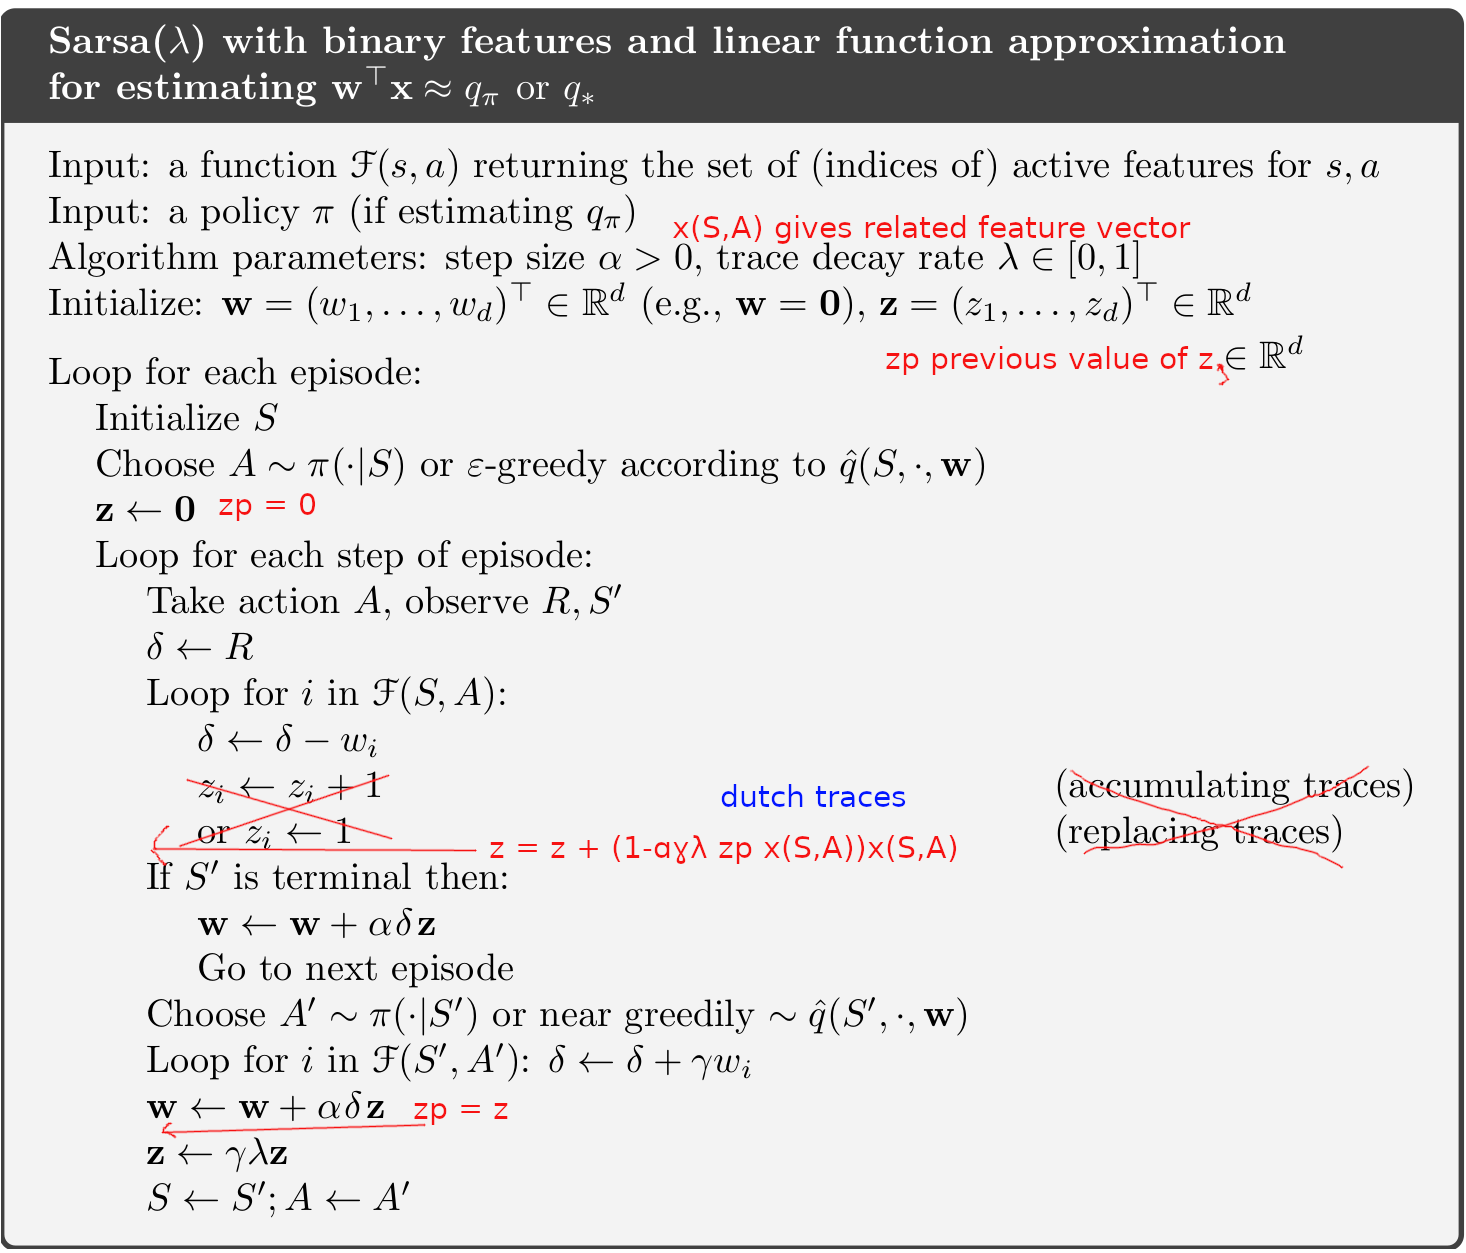
\includegraphics[scale=0.9]{exercise_12_6}

    \subsection{Question}

    Generalize the three recursive equations above to their truncated versions.

    \subsection*{Answer}

    Truncated versions of the recursive equations should be similar.
    However, recursion conditions have to change.
    Normally all components up to the end of episode are accumulating after fading as it is the case in figure 12.1.
    In the truncated version, only components up to min(t+n,T) should be accumulated as it the case in figure 12.7.
    Thus, recursive functions should terminate after returning:

        $ \lambda^{\begin{cases}%
  n-1       &   \text{if $t+n<T$}\\
  T-t-1     &   \text{ otherwise}
 \end{cases}} G_{t:\min(t+n,T)}^{\lambda} $

    \subsection{Question}

    Prove that (12.24) becomes exact if the value function does not change.
    To save writing, consider the case of t = 0, and use the notation

    \subsection*{Answer}

    \noindent Equation 12.22:

    \noindent $ G_{t}^{\lambda s} = \rho_{t} [ R_{t+1} \gamma_{t+1} ( (1-\lambda_{t+1}) \hat{v}_{t+1} +\lambda_{t+1}G_{t+1}^{\lambda s}) ] + (1-\rho_{t})\hat{v}_{t} $

    \hfill \break
    \noindent Start with removing the parenthesis:

    \noindent $ G_{t}^{\lambda s} = \rho_{t} [ R_{t+1} \gamma_{t+1} ( \hat{v}_{t+1} - \lambda_{t+1} \hat{v}_{t+1} + \lambda_{t+1}G_{t+1}^{\lambda s}) - \hat{v}_{t} ] + \hat{v}_{t} $

    \noindent $ G_{t}^{\lambda s} = \rho_{t} [ R_{t+1} + \gamma_{t+1} \hat{v}_{t+1} - \hat{v}_{t} + \gamma_{t+1} \lambda_{t+1} ( - \hat{v}_{t+1} + G_{t+1}^{\lambda s})  ] + \hat{v}_{t} $

    \noindent $ G_{t}^{\lambda s} = \rho_{t} [ \delta_{t} + \gamma_{t+1} \lambda_{t+1} ( - \hat{v}_{t+1} + G_{t+1}^{\lambda s})  ] + \hat{v}_{t} $

    \noindent $ G_{t}^{\lambda s} = \rho_{t} [ \delta_{t} + \gamma_{t+1} \lambda_{t+1} ( - \hat{v}_{t+1} +  \rho_{t+1} [ \delta_{t+1} + \gamma_{t+2} \lambda_{t+2} ( - \hat{v}_{t+2} + G_{t+2}^{\lambda s})  ] + \hat{v}_{t+1} )  ] + \hat{v}_{t} $

    \noindent $ G_{t}^{\lambda s} = \rho_{t} [ \delta_{t} + \gamma_{t+1} \lambda_{t+1} \rho_{t+1} [ \delta_{t+1} + \gamma_{t+2} \lambda_{t+2} ( - \hat{v}_{t+2} + G_{t+2}^{\lambda s})  ]  ] + \hat{v}_{t} $

    \noindent $ G_{t}^{\lambda s} = \rho_{t} [ \delta_{t} + \gamma_{t+1} \lambda_{t+1} \rho_{t+1} [ \delta_{t+1} + \gamma_{t+2} \lambda_{t+2} ( - \hat{v}_{t+2} + \rho_{t+2} [ \delta_{t+2} + \gamma_{t+3} \lambda_{t+3} ( - \hat{v}_{t+3} + G_{t+3}^{\lambda s})  ] + \hat{v}_{t+2} )  ]  ] + \hat{v}_{t} $

    \noindent $ G_{t}^{\lambda s} = \rho_{t} [ \delta_{t} + \gamma_{t+1} \lambda_{t+1} \rho_{t+1} [ \delta_{t+1} + \gamma_{t+2} \lambda_{t+2} \rho_{t+2} [ \delta_{t+2} + \gamma_{t+3} \lambda_{t+3} ( - \hat{v}_{t+3} + G_{t+3}^{\lambda s})  ]  ]  ] + \hat{v}_{t} $

    \hfill \break
    \noindent Distribute the leading coefficients to see the pattern:

    \noindent $ G_{t}^{\lambda s} = \rho_{t} \delta_{t} + \rho_{t} \gamma_{t+1} \lambda_{t+1} \rho_{t+1} [ \delta_{t+1} + \gamma_{t+2} \lambda_{t+2} \rho_{t+2} [ \delta_{t+2} + \gamma_{t+3} \lambda_{t+3} ( - \hat{v}_{t+3} + G_{t+3}^{\lambda s})  ]  ]  + \hat{v}_{t} $

    \noindent $ G_{t}^{\lambda s} = \rho_{t} \delta_{t} + \rho_{t} \gamma_{t+1} \lambda_{t+1} \rho_{t+1} \delta_{t+1} + \rho_{t} \gamma_{t+1} \lambda_{t+1} \rho_{t+1} \gamma_{t+2} \lambda_{t+2} \rho_{t+2} [ \delta_{t+2} + \gamma_{t+3} \lambda_{t+3} ( - \hat{v}_{t+3} + G_{t+3}^{\lambda s})  ]   + \hat{v}_{t} $

    \noindent $ G_{t}^{\lambda s} = \rho_{t} \delta_{t} + \rho_{t} \gamma_{t+1} \lambda_{t+1} \rho_{t+1} \delta_{t+1} + \rho_{t} \gamma_{t+1} \lambda_{t+1} \rho_{t+1} \gamma_{t+2} \lambda_{t+2} \rho_{t+2} \delta_{t+2} + \rho_{t} \gamma_{t+1} \lambda_{t+1} \rho_{t+1} \gamma_{t+2} \lambda_{t+2} \rho_{t+2} \gamma_{t+3} \lambda_{t+3} ( - \hat{v}_{t+3} + G_{t+3}^{\lambda s})   + \hat{v}_{t} $

    \noindent $ G_{t}^{\lambda s} = \delta_{t} \rho_{t} + \delta_{t+1} \rho_{t} \rho_{t+1} \gamma_{t+1} \lambda_{t+1} + \delta_{t+2} \rho_{t} \rho_{t+1} \rho_{t+2} \gamma_{t+1} \gamma_{t+2} \lambda_{t+1} \lambda_{t+2} + \rho_{t} \rho_{t+1} \rho_{t+2} \gamma_{t+1} \gamma_{t+2} \gamma_{t+3} \lambda_{t+1} \lambda_{t+2} \lambda_{t+3} ( - \hat{v}_{t+3} + G_{t+3}^{\lambda s})   + \hat{v}_{t} $

    \noindent $ G_{t}^{\lambda s} = \rho_{t} \sum_{k=t}^{\inf} \delta_{k} \prod_{i=t+1}^{k} \gamma_{i} \lambda_{i} \rho_{i} + \hat{v}_{t} $


    \subsection{Question}

    The truncated version of the general off-policy return is denoted G t:h .
    Guess the correct equation, based on (12.24).

    \subsection*{Answer}

    \noindent The truncated version of 12.24 should sum up to h instead of infinity.

    \noindent $ G_{t:h}^{\lambda s} = \rho_{t} \sum_{k=t}^{h} \delta_{k} \prod_{i=t+1}^{k} \gamma_{i} \lambda_{i} \rho_{i} + \hat{v}_{t} $

    \subsection{Question}

    Prove that (12.27) becomes exact if the value function does not change.
    To save writing, consider the case of t = 0, and use the notation Q k = q̂(S k , A k , w).
    Hint: Start by writing out 0 a and G 0 a , then G 0 a Q 0 .

    \subsection*{Answer}

    \noindent Equation 12.26:

    \noindent $ G_{t}^{\lambda a} = R_{t+1} + \gamma_{t+1} (\bar{V}_{t}(S_{t+1}) + \lambda_{t+1} \rho_{t+1} [ G_{t+1}^{\lambda a} -\hat{q}(S_{t+1},A_{t+1}, w_{t})] ) $

    \hfill \break
    \noindent Equation 12.28:

    \noindent $ \delta_{t}^{a} = R_{t+1} + \gamma_{t+1} \bar{V}_t(S_{t+1}) - \hat{q}(S_{t},A_{t}, w_{t}) ] $

    \hfill \break
    \noindent Following the hints:

    \noindent $ \delta_{0}^{a} = R_{1} + \gamma_{1} \bar{V}(S_{1}) - Q_{0} $

    \noindent $ G_{0}^{\lambda a} = R_{1} + \gamma_{1} (\bar{V}(S_{1}) + \lambda_{1} \rho_{1} [ G_{1}^{\lambda a} -Q_{1}] ) $

    \noindent $  G_{0}^{\lambda a} - Q_{0} = R_{1} + \gamma_{1} (\bar{V}(S_{1}) + \lambda_{1} \rho_{1} [ G_{1}^{\lambda a} -Q_{1}] ) -  Q_{0} $

    \noindent $  G_{0}^{\lambda a} - Q_{0} =  \delta_{0}^{a} + \gamma_{1} \lambda_{1} \rho_{1} [ G_{1}^{\lambda a} -Q_{1}] $

    \noindent $  G_{0}^{\lambda a} - Q_{0} =  \delta_{0}^{a} + \gamma_{1} \lambda_{1} \rho_{1} [   \delta_{1}^{a} + \gamma_{2} \lambda_{2} \rho_{2} [ G_{2}^{\lambda a} -Q_{2}]   ] $

    \hfill \break
    \noindent The pattern is visible:

    \noindent $  G_{0}^{\lambda a} - Q_{0} =  \sum_{k=0}^{\inf} \delta_{k}^{a} \prod_{i=t+1}^{k} \gamma_{i} \lambda_{i} \rho_{i} $

    \noindent $  G_{t}^{\lambda a} - Q_{t} =  \sum_{k=t}^{\inf} \delta_{k}^{a} \prod_{i=t+1}^{k} \gamma_{i} \lambda_{i} \rho_{i} $

    \noindent $  G_{t}^{\lambda a}  =   Q_{t} + \sum_{k=t}^{\inf} \delta_{k}^{a} \prod_{i=t+1}^{k} \gamma_{i} \lambda_{i} \rho_{i} $


    \subsection{Question}

    The truncated version of the general off-policy return is denoted G t:h.
    Guess the correct equation for it, based on (12.27).

    \subsection*{Answer}

    \noindent $  G_{t:h}^{\lambda a}  =   Q_{t} + \sum_{k=t}^{h} \delta_{k}^{a} \prod_{i=t+1}^{k} \gamma_{i} \lambda_{i} \rho_{i} $


    \subsection{Question}

    Show in detail the steps outlined above for deriving (12.29) from (12.27).
    Start with the update (12.15), substitute $G_{t}^{\lambda a}$ a from (12.26) for $G_{t}^{\lambda}$ , then follow similar steps as led to (12.25).

    \subsection*{Answer}

    \noindent Equation 12.27:

    \noindent $  G_{t}^{\lambda a}  =   Q_{t} + \sum_{k=t}^{\inf} \delta_{k}^{a} \prod_{i=t+1}^{k} \gamma_{i} \lambda_{i} \rho_{i} $

    \hfill \break
    \noindent Following the hints:

    \noindent $ w_{t+1} = w_{t} + \alpha [ G_{t}^{\lambda} - Q_{t}] \nabla Q_{t} $ t=0,1,\ldots,T-1 Equation 12.15

    \noindent $ w_{t+1} = w_{t} + \alpha [ G_{t}^{\lambda a} - Q_{t}] \nabla Q_{t} $ t=0,1,\ldots,T-1 Equation 12.15

    \noindent $ w_{t+1} = w_{t} + \alpha [Q_{t} + \sum_{k=t}^{\inf} \delta_{k}^{a} \prod_{i=t+1}^{k} \gamma_{i} \lambda_{i} \rho_{i} - Q_{t}] \nabla Q_{t} $ t=0,1,\ldots,T-1 Equation 12.15

    \noindent $ w_{t+1} = w_{t} + \alpha [\sum_{k=t}^{\inf} \delta_{k}^{a} \prod_{i=t+1}^{k} \gamma_{i} \lambda_{i} \rho_{i}] \nabla Q_{t} $ t=0,1,\ldots,T-1 Equation 12.15

    \hfill \break
    \noindent The sum of the forward-view update over time is:

    \noindent $ \sum_{t=1}^{\infty} (w_{t+1} - w_t) = \sum_{t=1}^{\infty} \sum_{k=t}^{\infty} \alpha  \delta_{k}^{a} \nabla Q_{t} \prod_{i=t+1}^{k} \gamma_{i} \lambda_{i} \rho_{i}  $

    \noindent $ \sum_{t=1}^{\infty} (w_{t+1} - w_t) = \sum_{k=1}^{\infty} \sum_{t=1}^{k} \alpha  \delta_{k}^{a} \nabla Q_{t} \prod_{i=t+1}^{k} \gamma_{i} \lambda_{i} \rho_{i}  $ by summation rule $ \sum_{t=x}^{y} \sum_{k=t}^{y} = \sum_{k=x}^{y} \sum_{t=x}^{k}  $

    \noindent $ \sum_{t=1}^{\infty} (w_{t+1} - w_t) = \sum_{k=1}^{\infty} \alpha  \delta_{k}^{a} \sum_{t=1}^{k} \nabla Q_{t} \prod_{i=t+1}^{k} \gamma_{i} \lambda_{i} \rho_{i}  $

    \noindent $ z_k = \sum_{t=1}^{k} \nabla Q_{t} \prod_{i=t+1}^{k} \gamma_{i} \lambda_{i} \rho_{i}  $

    \noindent $ z_k = \sum_{t=1}^{k-1} \nabla Q_{t} \prod_{i=t+1}^{k} \gamma_{i} \lambda_{i} \rho_{i} + \nabla Q_{k} $

    \noindent $ z_k = \gamma_{k} \lambda_{k} \rho_{k} [ \sum_{t=1}^{k-1} \nabla Q_{t} \prod_{i=t+1}^{k-1} \gamma_{i} \lambda_{i} \rho_{i} ] + \nabla Q_{k} $

    \noindent $ z_k = \gamma_{k} \lambda_{k} \rho_{k} z_{k-1} + \nabla Q_{k} $

    \noindent $ z_t = \gamma_{t} \lambda_{t} \rho_{t} z_{t-1} + \nabla Q_{t} $

    \subsection{Question}

    What are the dutch-trace and replacing-trace versions of off-policy eligibility traces for state-value and action-value methods?

    \subsection*{Answer}

    \noindent My dutch-trace guesses are:

    \noindent $ z_t = \rho_{t} (\gamma_{t} \lambda_{t} z_{t-1} + (1-\alpha \gamma_t \lambda_t z_{t-1} x_t)x_t ) $

    \noindent $ z_t = \gamma_{t} \lambda_{t} \rho_{t} z_{t-1} + (1-\alpha \gamma_t \lambda_t z_{t-1} \rho_{t} x_t)x_t $

    \hfill \break
    \noindent My replacing-trace guesses are (the replacing traces are defined for binary features):

    \noindent $ z_{t,i} = \rho_{t} (\gamma_{t} \lambda_{t} z_{t-1} (1- x_{t,i}) + x_{t,i} ) $

    \noindent $ z_{t,i} = \gamma_{t} \lambda_{t} \rho_{t} z_{t-1} (1- x_{t,i}) + \rho_{t} x_{t,i} $

    \subsection{Question}

    What are the dutch-trace and replacing-trace versions of off-policy eligibility traces for state-value and action-value methods?

    \subsection*{Answer}

    \noindent Semi gradient parameter update rule (12.7)

    \noindent $ w_{t+1} = w_{t} + \alpha \delta_{t} z_{t} $

    \hfill \break
    \noindent Dutch trace (12.11):

    \noindent $ z_t = \lambda \gamma z_{t-1} + (1-\alpha \gamma \lambda z_{t-1}^{T} x_t) x_t $

    \hfill \break
    \noindent Expectation based TD error (12.28)

    \noindent $ \delta_{t}^{a} = R_{t+1} + \gamma_{t+1} \bar{V}_{t}(S_{t+1}) - \hat{q}(S_t,A_t,w_t) $


    \hfill \break
    \noindent Expectation approximate value function (12.21)

    \noindent $ \bar{V}_{t}(s) = \sum_{a} \pi(a|s)\hat{q}(s,a,w)  $


    \hfill \break
    \noindent Slightly modify 12.21:

    \noindent $ \bar{V}_{k, t}(s) = \sum_{a} \pi_{k}(a|s)\hat{q}(s,a,w_{k})  $

    \hfill \break
    \noindent In double expected SARSA there will be two policy to select actions $\pi_1$ and $\pi_2$  with their respective action value functions $Q_1$ and $Q_2$. (From exercise 6.12)

    \noindent $ Q_1(S_t, A_t) =  Q_1(S_t, A_t) + \alpha [ R_{t+1} + \gamma E_{\pi_2} [ Q_2(S_{t+1}, A_{t+1}) | S_{t+1}] - Q_1(S_t, A_t) ] $

    \noindent $ Q_2(S_t, A_t) =  Q_2(S_t, A_t) + \alpha [ R_{t+1} + \gamma E_{\pi_1} [ Q_1(S_{t+1}, A_{t+1}) | S_{t+1}] - Q_2(S_t, A_t) ] $

    \hfill \break
    \noindent After combining all the available data, the update rules should look like:

    \noindent $ w_{1, t+1} = w_{1, t} + \alpha (R_{t+1} + \gamma_{t+1} \bar{V}_{2, t}(S_{t+1}) - \hat{q}(S_t,A_t,w_{1,t}))  z_{t} $

    \noindent $ w_{2, t+1} = w_{2, t} + \alpha (R_{t+1} + \gamma_{t+1} \bar{V}_{1, t}(S_{t+1}) - \hat{q}(S_t,A_t,w_{2,t}))  z_{t} $


\end{document}


